\section{SEDflow} \label{sec:sedflow}
In this work we apply ANPE to SED modeling of galaxy spectra. 
tl;dr of intro 

\subsection{SED Modeling: PROVABGS} \label{sec:provabgs}
% section explaining specific SED set up 

provabgs set up 

\subsection{Training} \label{sec:training}
paragraph describing the training data
\begin{itemize}
    \item noise model 
\end{itemize}

description of the ANPE training
\begin{itemize}
    \item architecture
    \item validation 
\end{itemize}

\begin{figure}
\begin{center}
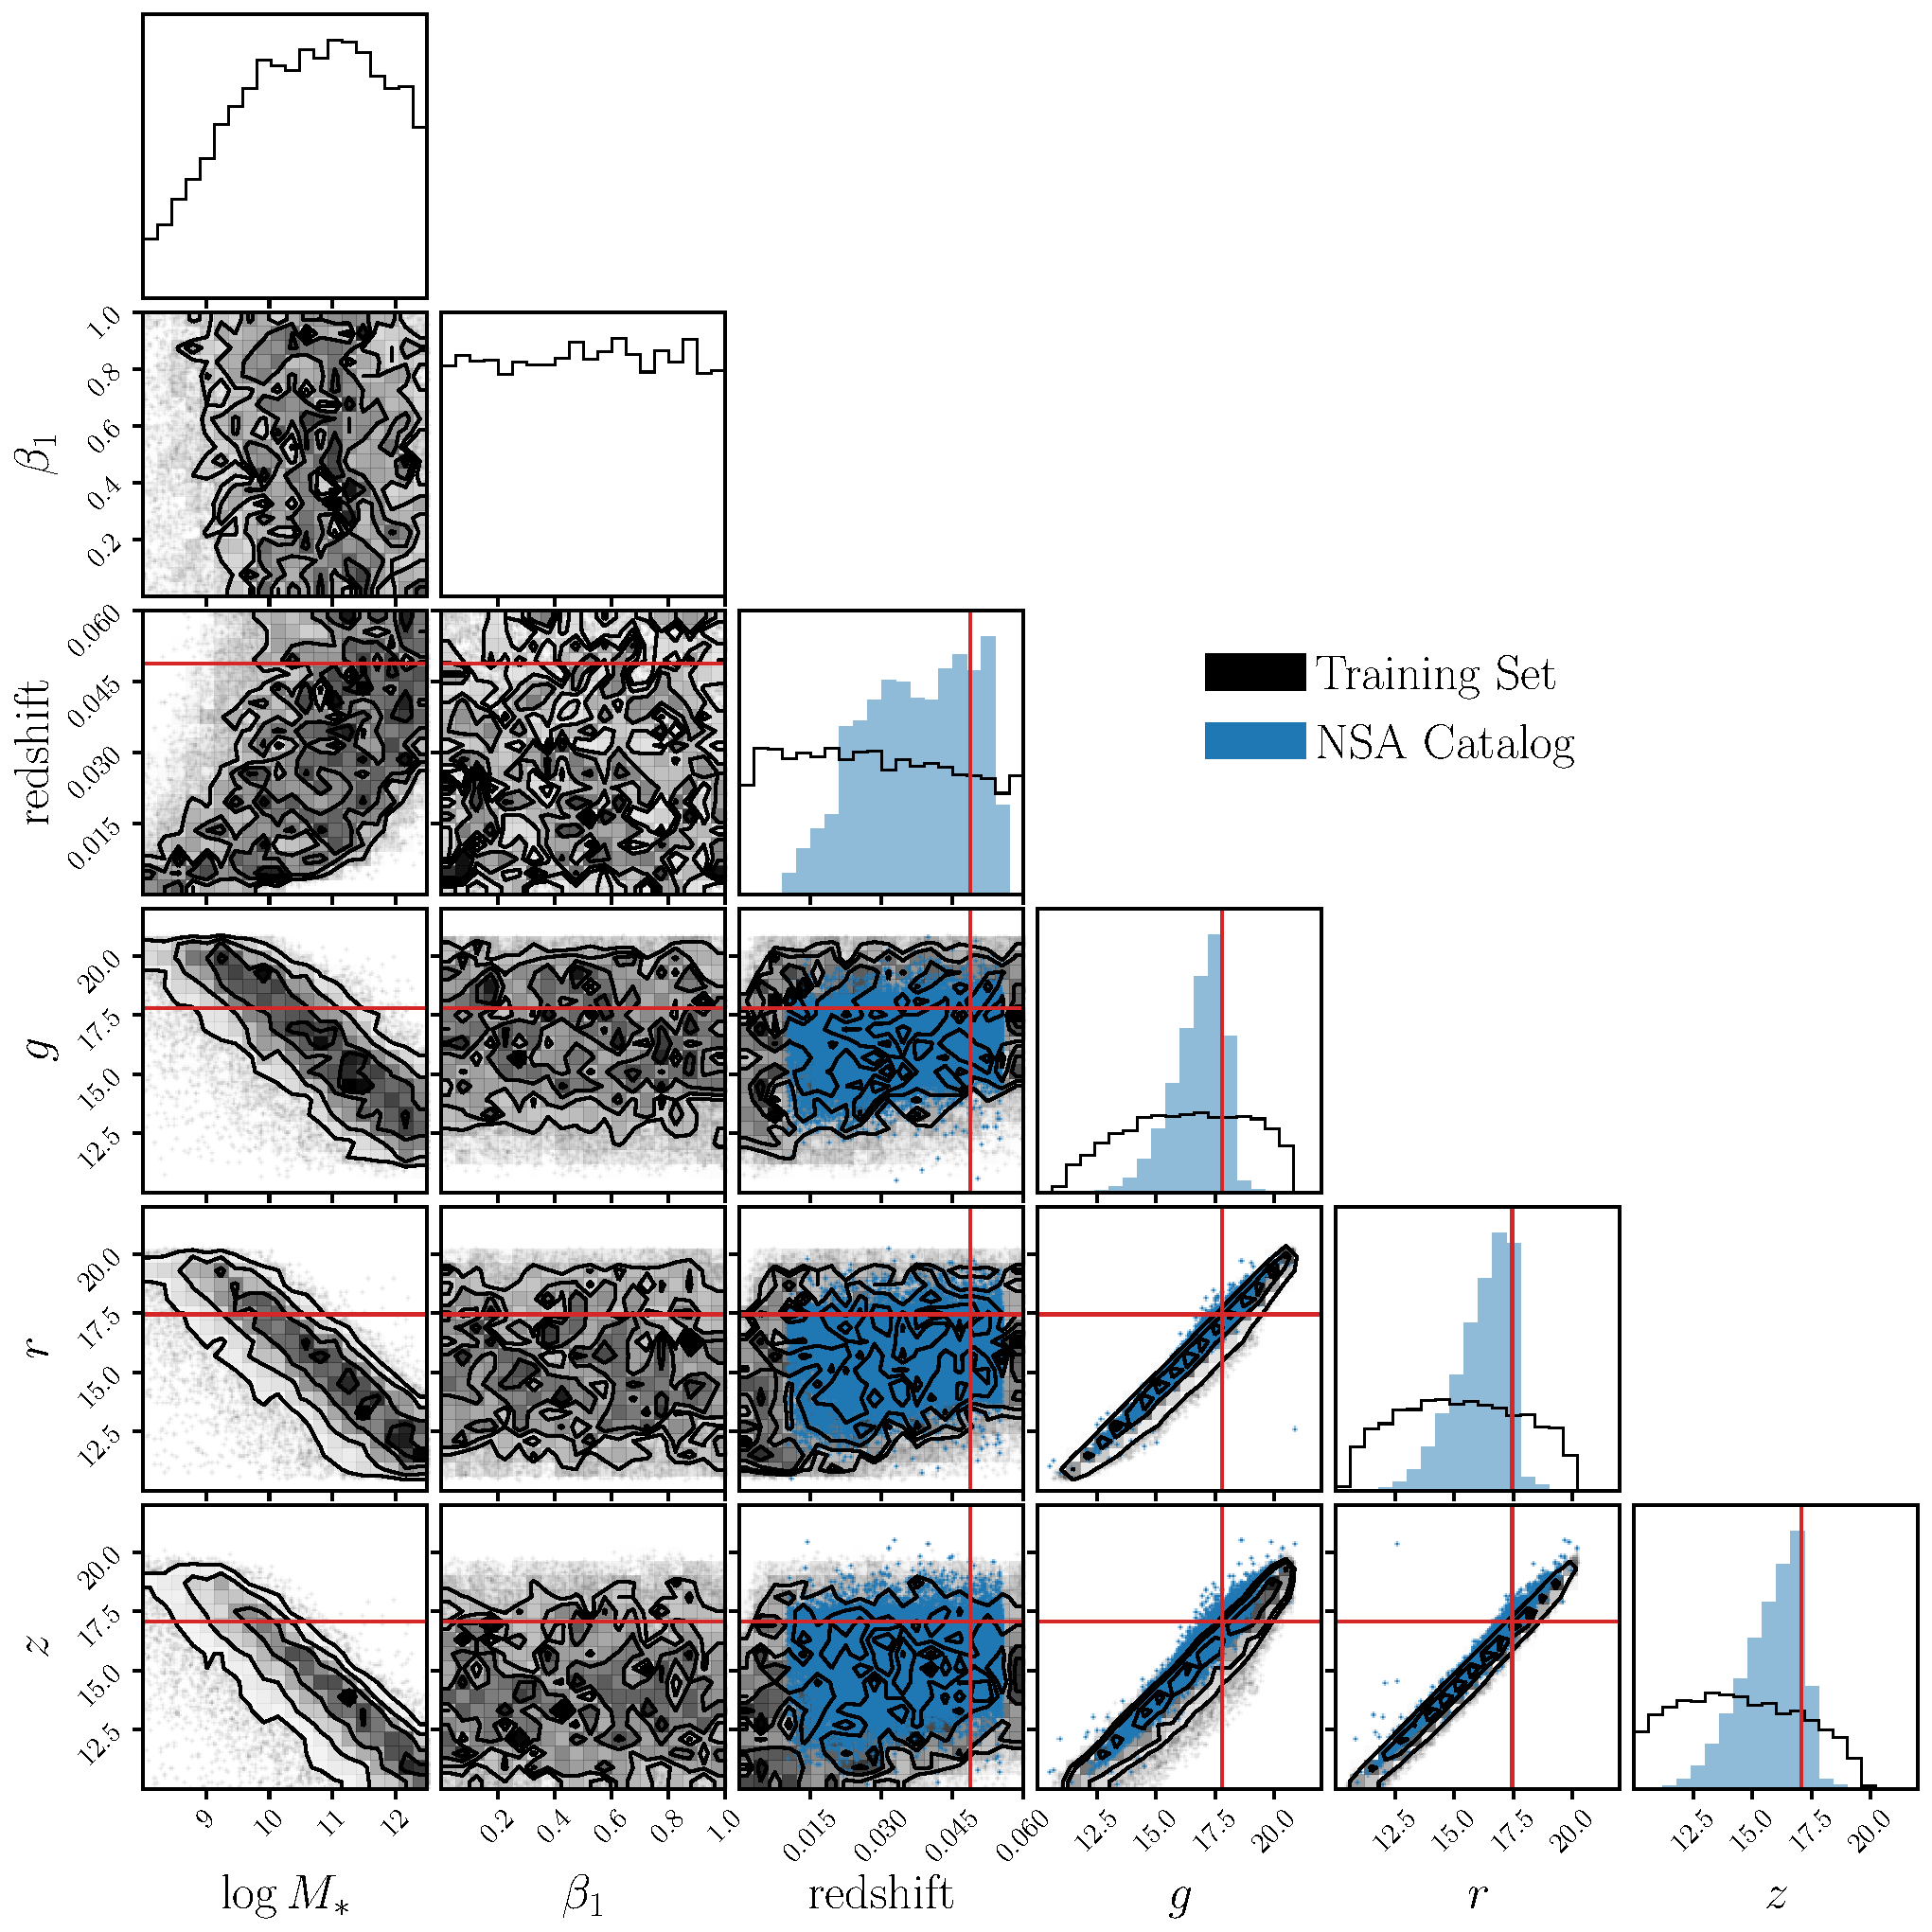
\includegraphics[width=0.9\textwidth]{figs/training.pdf}
    \caption{\label{fig:data}
    Joint distribution of SED model parameters ($\log M_*$, $\beta_1$,
    redshift) and photometric magnitudes ($g$, $r$, $z$) for our training set.
    The training set was constructed by sampling parameter values from the
    prior (Table~\ref{tab:prior}), constructing SEDs using a theoretical SPS
    model, and applying our noise model. 
    For details, we refer readers to Section~\ref{sec:sbi_sed}.
    For comparison, we present the distribution of magnitudes for galaxies in
    the NSA catalog (blue). 
    \emph{The training set fully encompasses the observations, thus, our 
    {\sc SEDflow} method can be used to infer the posterior for all NSA
    galaxies}.
    }
\end{center}
\end{figure}


